% Figure from MATH 591 notes, section 49. Compile with the notes preamble.
\begin{tikzpicture}[scale=1.1]
\draw[gray!45] (-2.6,0.35) rectangle (2.6,2.8);
\node[gray!70!black, font=\footnotesize, anchor=south west] at (-2.6,2.8) {$\mathbb{R}^2$};
\draw[gray!35, dashed] (-2.00,0.35) -- (-2.00,2.8);
\draw[->, thick, violet!75!black] (-2.000,0.750) -- (-1.819,0.539);
\draw[orange!80!black, densely dotted] (-2.000,0.750) -- (-1.819,0.750);
\draw[->, thick, violet!75!black] (-2.000,1.500) -- (-1.819,1.786);
\draw[orange!80!black, densely dotted] (-2.000,1.500) -- (-1.819,1.500);
\draw[->, thick, violet!75!black] (-2.000,2.250) -- (-1.819,2.627);
\draw[orange!80!black, densely dotted] (-2.000,2.250) -- (-1.819,2.250);
\draw[gray!35, dashed] (-1.00,0.35) -- (-1.00,2.8);
\draw[->, thick, violet!75!black] (-1.000,0.750) -- (-0.587,0.904);
\draw[orange!80!black, densely dotted] (-1.000,0.750) -- (-0.587,0.750);
\draw[->, thick, violet!75!black] (-1.000,1.500) -- (-0.587,1.919);
\draw[orange!80!black, densely dotted] (-1.000,1.500) -- (-0.587,1.500);
\draw[->, thick, violet!75!black] (-1.000,2.250) -- (-0.587,2.340);
\draw[orange!80!black, densely dotted] (-1.000,2.250) -- (-0.587,2.250);
\draw[gray!35, dashed] (0.00,0.35) -- (0.00,2.8);
\draw[->, thick, violet!75!black] (0.000,0.750) -- (0.500,1.152);
\draw[orange!80!black, densely dotted] (0.000,0.750) -- (0.500,0.750);
\draw[->, thick, violet!75!black] (0.000,1.500) -- (0.500,1.734);
\draw[orange!80!black, densely dotted] (0.000,1.500) -- (0.500,1.500);
\draw[->, thick, violet!75!black] (0.000,2.250) -- (0.500,1.985);
\draw[orange!80!black, densely dotted] (0.000,2.250) -- (0.500,2.250);
\draw[gray!35, dashed] (1.00,0.35) -- (1.00,2.8);
\draw[->, thick, violet!75!black] (1.000,0.750) -- (1.413,1.096);
\draw[orange!80!black, densely dotted] (1.000,0.750) -- (1.413,0.750);
\draw[->, thick, violet!75!black] (1.000,1.500) -- (1.413,1.373);
\draw[orange!80!black, densely dotted] (1.000,1.500) -- (1.413,1.500);
\draw[->, thick, violet!75!black] (1.000,2.250) -- (1.413,1.830);
\draw[orange!80!black, densely dotted] (1.000,2.250) -- (1.413,2.250);
\draw[gray!35, dashed] (2.00,0.35) -- (2.00,2.8);
\draw[->, thick, violet!75!black] (2.000,0.750) -- (2.181,0.778);
\draw[orange!80!black, densely dotted] (2.000,0.750) -- (2.181,0.750);
\draw[->, thick, violet!75!black] (2.000,1.500) -- (2.181,1.107);
\draw[orange!80!black, densely dotted] (2.000,1.500) -- (2.181,1.500);
\draw[->, thick, violet!75!black] (2.000,2.250) -- (2.181,1.993);
\draw[orange!80!black, densely dotted] (2.000,2.250) -- (2.181,2.250);
\draw[->, thick, gray!70] (3.0,1.45) -- node[right, font=\scriptsize] {$\pi$} (3.0,0.05);
\draw[thick, gray!70] (-2.6,-0.45) -- (2.6,-0.45) node[right, font=\footnotesize, text=black] {$\mathbb{R}$};
\fill (-2.00,-0.45) circle (1.2pt);
\draw[->, very thick, orange!85!black] (-2.000,-0.45) -- (-1.819,-0.45);
\fill (-1.00,-0.45) circle (1.2pt);
\draw[->, very thick, orange!85!black] (-1.000,-0.45) -- (-0.587,-0.45);
\fill (0.00,-0.45) circle (1.2pt);
\draw[->, very thick, orange!85!black] (0.000,-0.45) -- (0.500,-0.45);
\fill (1.00,-0.45) circle (1.2pt);
\draw[->, very thick, orange!85!black] (1.000,-0.45) -- (1.413,-0.45);
\fill (2.00,-0.45) circle (1.2pt);
\draw[->, very thick, orange!85!black] (2.000,-0.45) -- (2.181,-0.45);
\node[violet!75!black, font=\scriptsize, align=left, anchor=west] at (3.5,2.05) {$\mathbf{X} = b(x)\,\partial_x + (\text{anything})\,\partial_y$};
\node[orange!80!black, font=\scriptsize, align=left, anchor=west] at (3.5,1.55) {dotted: the horizontal part $b(x)$,\\ the same all along each fibre};
\node[orange!85!black, font=\scriptsize, anchor=west] at (3.5,-0.45) {$\mathbf{Y} = b(x)\,\dfrac{d}{dx}$};
\end{tikzpicture}
